    \begin{subfigure}[c]{0.4\textwidth}
        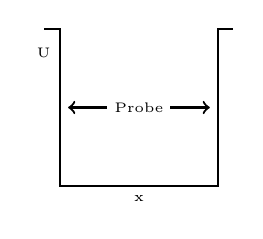
\begin{tikzpicture}
            % Potential
            \draw (1,1) node {\tiny Probe};
            \draw [thick] [<-](0.1,1) -- (0.6,1);
            \draw [thick] [->] (1.4,1) -- (1.9,1);
            \draw [thick]%
            (-0.2,2) -- (0,2) -- (0,0) -- (2,0) -- (2,2) -- (2.2,2);
            \draw (1,0) node[anchor=north] {\tiny x};
            \draw (0,1.7) node[anchor=east] {\tiny U};
        \end{tikzpicture}
        \caption{Potentialverlauf der Probe}
    \end{subfigure}
    \begin{subfigure}[c]{0.4\textwidth}
        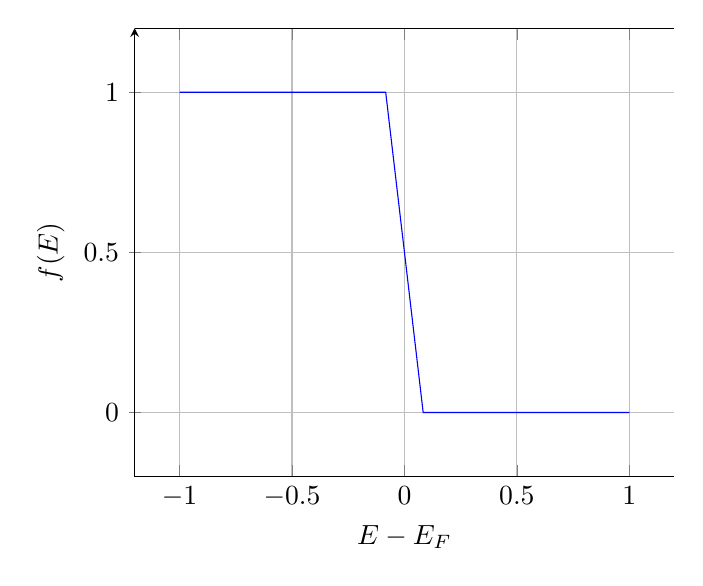
\begin{tikzpicture}
            \begin{axis}[%
                    xlabel={$E-E_F$},
                    ylabel={$f(E)$},
                    domain=-1:1,
                    ymin=-0.2,
                    ymax=1.2,
                    axis y line=left,
                    grid=both
            ]
                \addplot[color=blue]%
                {1/(exp(x/0.00086)+1)};
            \end{axis}
        \end{tikzpicture}
        \caption{Zustandsverteilung im Elektronengas}
    \end{subfigure}
